\documentclass[a4paper, 10pt,onecolumn]{scrartcl}
\usepackage[ngerman]{babel}
\usepackage[T1]{fontenc}
\usepackage[utf8]{inputenc}
\usepackage{multirow}
\usepackage{natbib}
\usepackage{graphicx}
\usepackage{amsmath, amssymb}
\usepackage{grffile} %einfacheres einbinden von Dateipfaden
\usepackage{hyperref}


\title{Schlechte Bilder\thanks{Danke an John Wigg}} 
\author{Ich} %auch nach \begindocument möglich
\date{\today}
\setlength{\parindent}{0pt}

\begin{document}
\tableofcontents
\listoffigures

\section{Autokorrelation }
\subsection{Definition}

Die quadratische interferometrische Autokorrelationsfunktion $S_{quadAC}(\tau)$, definiert als
\begin{center}
	\begin{equation}
		S_{quadAC}(\tau)=\int_{-\infty}^{\infty}[E(t)+E(t-\tau)]^4\mathrm{d}t
		\label{eq:formel}
	\end{equation}
\end{center}
kann z.\,B. genutzt werden, um kurze Pulse zu analysieren. Wie man in Gleichung \eqref{eq:formel} sehen kann muss man für die Autokorrelation von $-\infty$ bis $\infty$ integrieren.

\subsection{Messung}
Tabelle \ref{Tabelle1} zeigt Messungen der Autokorrelation.
\begin{table}[h!]
\centering
\caption{Autokorrelation zu den Zeitpunkten $\tau =0$  und $\tau=\tau_1$}
\label{Tabelle1}
\begin{tabular}{|c|c|}
\hline \hline
$S_{quadAC}(0)$ & $S_{quadAC}(\tau_1)$\\ \hline
$0.001 V^4sm^{-4}$ & $0.32 V^4sm^{-4}$\\ \hline \hline
\end{tabular}
\end{table}
\section{Ionenerträge}

In \ref{Tabelle2} (auf Seite 2) sind Ionenerträge aufgeführt. Die Tabelle ist dem Artikel [1] entnommen und leicht verändert.

\begin{table}[!h]
\centering
\caption{Relative Ionenerträge nach resonanter 1$s^{-1}3p-$ Anregung in Neon. Neben den berechneten Werten sind die experimentellen Daten von Morgan $et al.$ [2] aufgeführt.}
\label{Tabelle2}
\begin{tabular}{ccc}
\hline \hline
&\multicolumn{2}{c}{Ionenerträge}\\ \cline{2-3}
Ion & Theorie & Exp. [2] \\ \hline
N$e^1+$ & 0.74 & 0.65 $\pm$ 0.02\\
N$e^2+$ & 0.26 & 0.31 $\pm$ 0.02 \\ 
N$e^3+$ & -- & 0.03 $\pm$ 0.01\\
N$e^4+$ & -- & 0.002\\
\hline \hline

\end{tabular}
\end{table}

\begin{figure}
\centering
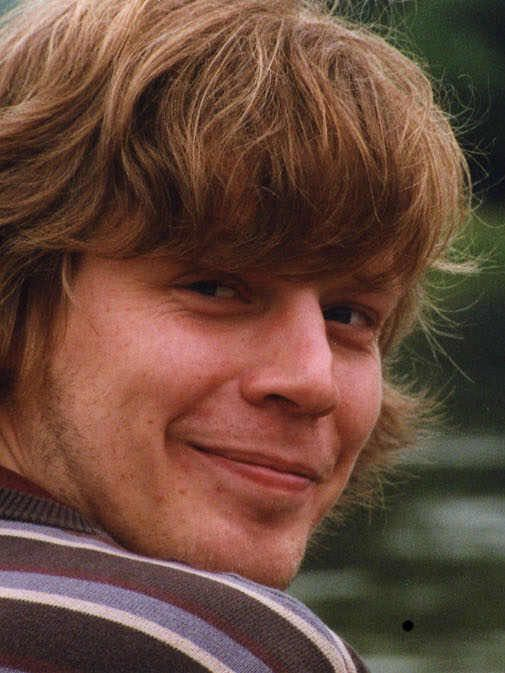
\includegraphics[scale=0.25]{tauti.jpg}
\caption{Nicht die Sombrero Galaxie (M 104)}
\end{figure}

\section{Nicht die Sombrero-Galaxie}

Dieser Abschnitt hat nichts zu tun mit den Tabellen \ref{Tabelle1} und \ref{Tabelle2} oder der Gleichung \eqref{eq:formel}. Er handelt nicht von der Sombrero-Galaxie, Objekt Nummer M 104 im Messier-Katalog. Ein Bild der Galaxie kann in Abb. \ref{Tabelle1} auf Seite 2 bestaunt werden.





\end{document}
